\newpage
\section{Билет 24. Отказоустойчивость. Активная и пассивная репликация. Алгоритмы поддержания согласованного состояния реплик. Построение надежного хранилища из ненадежных компонентов.}

Отказоустойчивость — свойство технической системы сохранять свою работоспособность после отказа одной или нескольких её составных частей. Отказоустойчивость определяется количеством единичных отказов составных частей (элементов) системы, после наступления которых сохраняется работоспособность системы в целом. Базовый уровень отказоустойчивости подразумевает защиту от отказа одного любого элемента, однако в теории можно реализовать систему с практическим любым количеством отказов.

\if (0)
Для сохранения данных в случае отказа каких-то из частей системы (сервера/кластера/ПК...) используется несколько приемов:
\begin{itemize}
	\item Репликация -- создание нескольких одинаковых систем, к которым направляются одинаковые задачи. Результат выполнения задач определяется <<голосованием>>. Данный подход включает в себя обмен информацией, чтобы обеспечить согласованность между системами, для повышения надежности, отказоустойчивости.
	\item Избыточность -- создание нескольких одинаковых систем с целью повышения надежности системы, обычно в форме резервного копирования или отказоустойчивости. В случае отказа одной из частей другие части включаются в работу.
	\item Разнообразие (Diversity): Создание 
\end{itemize}
\fi

Примером отказоустойчивой систем является RAID(\url{https://ru.wikipedia.org/wiki/RAID}).

\subsection{Активная и пассивная репликации.}
В построении отказоустойчивых систем есть два главных подхода к проектированию: активная и пассивная репликация.

\textbf{Активная репликация ((State Machine Approach)} - каждый элемент (реплика) системы хранит копию состояния данных. Операции чтения и модификации выполняются локально в каждом узле. Для поддержания когерентности реплик операции модификации рассылаются всем репликам объекта, которые выполняют их над локальной копией состояния. При выходе из строя части реплик проводиться <<голосование>> для выбора <<главной>> реплики. Например с помощью следующих алгоритмов: протокол «Византийского соглашения» \url{https://clck.ru/JVS7z}, R-Broadcast ~\ref{b19:part2}, алгоритма Консенсуса). Для клиента из вне вся система выглядит как один сервер. Отсутствует централизованный контроль, однако в процессе работы выполняется много избыточных вычислений и коммуникаций.
\begin{figure}[H]
	\centering
	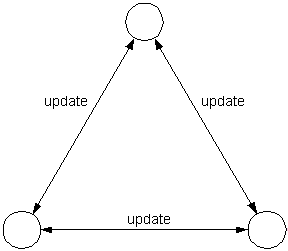
\includegraphics[scale = 0.7]{24/active.png}
	\caption{Схема активной репликации}
	\label{fig:active_repl}
\end{figure}

\textbf{Пассивная репликация} - каждый элемент (реплика) системы хранит копию состояния данных. Одна из реплик назначается главной. Операции чтения выполняются локально во всех узлах. Операции, модифицирующие состояние объекта, направляются главной реплике, которая, после выполнения метода, обновляет все остальные реплики. При выводе из строя главной реплики пользователь замечает проблемы с доступом к данным, до тех пор пока одна из запасных реплик не возьмет на себя роль главной. Данный метод обладает намного меньшим потреблением ресурсов и отсутствие большого количества избыточных коммуникаций и вычислений в сравнении с активной репликацией, и поэтому используется чаще.
\begin{figure}[H]
	\centering
	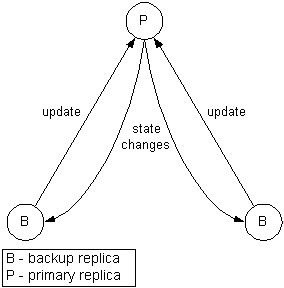
\includegraphics[scale = 0.7]{24/passive.png}
	\caption{Схема пассивной репликации}
	\label{fig:passive_repl}
\end{figure}



	
